\documentclass[a4paper,14pt]{extarticle}

\usepackage[utf8x]{inputenc}
\usepackage[T1,T2A]{fontenc}
\usepackage[russian]{babel}
\usepackage{hyperref}
\usepackage{indentfirst}
\usepackage{here}
\usepackage{array}
\usepackage{graphicx}
\usepackage{caption}
\usepackage{subcaption}
\usepackage{chngcntr}
\usepackage{amsmath}
\usepackage{amssymb}
\usepackage{pgfplots}
\usepackage{pgfplotstable}
\usepackage[left=2cm,right=2cm,top=2cm,bottom=2cm,bindingoffset=0cm]{geometry}
\usepackage{multicol}
\usepackage{askmaps}
\usepackage{enumitem}

\setitemize{itemsep=0em}
\setenumerate{itemsep=0em}

\renewcommand{\le}{\ensuremath{\leqslant}}
\renewcommand{\leq}{\ensuremath{\leqslant}}
\renewcommand{\ge}{\ensuremath{\geqslant}}
\renewcommand{\geq}{\ensuremath{\geqslant}}
\renewcommand{\epsilon}{\ensuremath{\varepsilon}}
\renewcommand{\phi}{\ensuremath{\varphi}}
\renewcommand{\thefigure}{\arabic{figure}} 	
\renewcommand*\not[1]{\overline{#1}}

%\titleformat*{\section}{\large\bfseries} 
%\titleformat*{\subsection}{\normalsize\bfseries} 
%\titleformat*{\subsubsection}{\normalsize\bfseries} 
%\titleformat*{\paragraph}{\normalsize\bfseries} 
%\titleformat*{\subparagraph}{\normalsize\bfseries} 

\counterwithin{figure}{section}
\counterwithin{equation}{section}
\counterwithin{table}{section}
\newcommand{\sign}[1][5cm]{\makebox[#1]{\hrulefill}}
\graphicspath{{../pics/}}
\captionsetup{justification=centering,margin=1cm}
\def\arraystretch{1.3}
\setlength\parindent{5ex}
%\titlelabel{\thetitle.\quad}

\begin{document}

\begin{titlepage}
\begin{center}
	Санкт-Петербургский Политехнический Университет Петра Великого\\[0.3cm]
	Институт компьютерных наук и технологий \\[0.3cm]
	Кафедра компьютерных систем и программных технологий\\[4cm]
	
	\textbf{ОТЧЕТ}\\ 
	\textbf{по лабораторной работе}\\[0.5cm]
	\textbf{<<Исследование персептронов>>}\\[0.1cm]
	\textbf{Нейроинформатика}\\[4.0cm]
\end{center}

\begin{flushright}
	\begin{minipage}{0.45\textwidth}
		\textbf{Работу выполнил студент}\\[3mm]
		группа 33501/4 \hspace*{10mm} Дьячков В.В.\\[5mm]
		\textbf{Преподаватель}\\[5mm]
		\sign[1.7cm] \hspace*{1mm} к.т.н., доц. Никитин К.В. \\[5mm]
	\end{minipage}
\end{flushright}

\vfill

\begin{center}
	Санкт-Петербург\\
	\the\year
\end{center}
\end{titlepage}

\addtocounter{page}{1}

\tableofcontents
\newpage
\listoffigures
\newpage

\section{Цели работы}

Изучение архитектуры персептрона и специальных функций для создания персептрона, настройки его весов и смещений и адаптации, ознакомление с демонстрационными примерами, а так­же приобретение навыков построения и обучения персептронов для различных областей применения.

\section{Классификация 2 линейно-неразделимых классов}

\subsection{Набор входных и желаемых образов}

%1. Сформируйте набор входных и желаемых выходных образов ( “0” – класс 1, “X” – класс 2. Постройте график и нанесите на него эти точки.

Сформируем набор входных и желаемых выходных образов для двух линейно-неразделимых классов. На рис. \ref{fig:1_1} входной набор изоражен на графике, при этом класс \verb+0+ отмечен синими кругами, а класс \verb+1+ красными крестиками.

\begin{figure}[H]
\begin{center}
	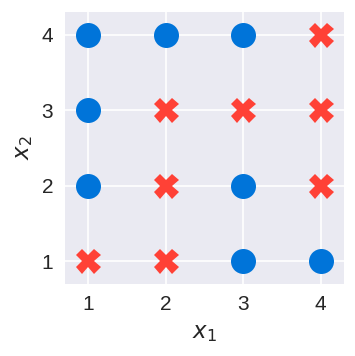
\includegraphics[scale=1.1]{1_1}
	\caption{Набор выходных и желаемых выходных образов}
	\label{fig:1_1}
\end{center}
\end{figure}

\subsection{Аналитическое решение}

%2. Для заданного варианта сформируйте собственный вариант решения задачи без ошибок и реализуйте его аналитически вначале математически с помощью формул, а затем с помощью 2-х или 3-х слойного персептрона (для этого вначале с помощью кусочно-линейной аппроксимации задайте функции, определяющие принадлежность к классу 1 и 2). 

Разделим входное пространство на 4 выпуклые области, ограниченные прямыми:
\begin{equation*}
	\begin{cases}
		>1\\
		>2
	\end{cases}
	\hspace{1cm}
	\begin{cases}
		<3\\
		>4\\
		>5
	\end{cases}
	\hspace{1cm}
	\begin{cases}
		<3\\
		>4\\
		<6
	\end{cases}
	\hspace{1cm}
	\begin{cases}
		<6\\
		<7
	\end{cases}
\end{equation*}

\begin{figure}[H]
\begin{center}
	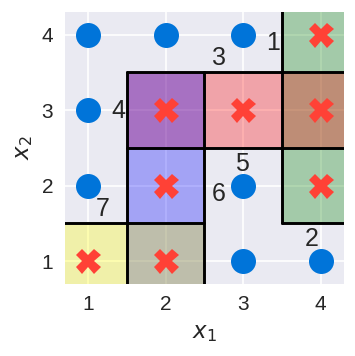
\includegraphics[scale=1.1]{1_2_1}
	\caption{Разбие с помощью множества прямых}
	\label{fig:1_2_1}
\end{center}
\end{figure}

Составим уравнения прямых для каждого слоя:

\paragraph{Первый слой}
\begin{enumerate}
	\item $x_1 - 3.5 = 0 \rightarrow y_{11}$
	\item $x_2 - 1.5 = 0 \rightarrow y_{12}$
	\item $-x_2 + 3.5 = 0 \rightarrow y_{13}$
	\item $x_1 - 1.5 = 0 \rightarrow y_{14}$
	\item $x_2 - 2.5 = 0 \rightarrow y_{15}$
	\item $-x_1 + 2.5 = 0 \rightarrow y_{16}$
	\item $-x_2 + 1.5 = 0 \rightarrow y_{17}$
\end{enumerate}

\paragraph{Второй слой}
\begin{enumerate}
	\item $y_{11} + y_{12} - 1.5 = 0 \rightarrow y_{21}$
	\item $y_{13} + y_{14} + y_{15} - 2.5 = 0 \rightarrow y_{22}$
	\item $y_{13} + y_{14} + y_{16} - 2.5 = 0 \rightarrow y_{23}$
	\item $y_{16} + y_{17} - 1.5 = 0 \rightarrow y_{24}$
\end{enumerate}

\paragraph{Третий слой}
\begin{enumerate}
	\item $y = y_{21} + y_{22} + y_{23} + y_{24} - 0.5$
\end{enumerate}

\begin{figure}[H]
\begin{center}
	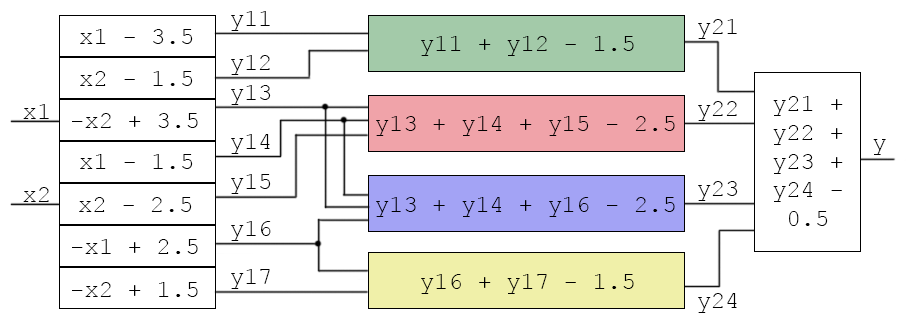
\includegraphics[width=\textwidth]{1_2_2}
	\caption{Аналитическое разбиение}
	\label{fig:1_2_2}
\end{center}
\end{figure}

\subsection{Схема сети}

%3. Сгенерируйте схему командой gensim (net), проанализируйте ее и приведите в отчет.

На рис. \ref{fig:1_3} изображена схема, полученная при помощи команды \verb+gensim+.

\begin{figure}[H]
\begin{center}
	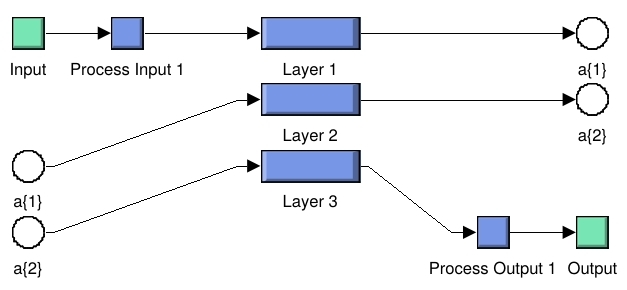
\includegraphics[width=0.7\textwidth]{1_3}
	\caption{Схема сети}
	\label{fig:1_3}
\end{center}
\end{figure}

\subsection{Проверка аналитического разбиения}

%4. Проверьте полученные функции в заданных точках, а также в близлежащих точках.

На рис. \ref{fig:1_4} изображено разбиение случайных точек входного пространства на классы.

\begin{figure}[H]
\begin{center}
	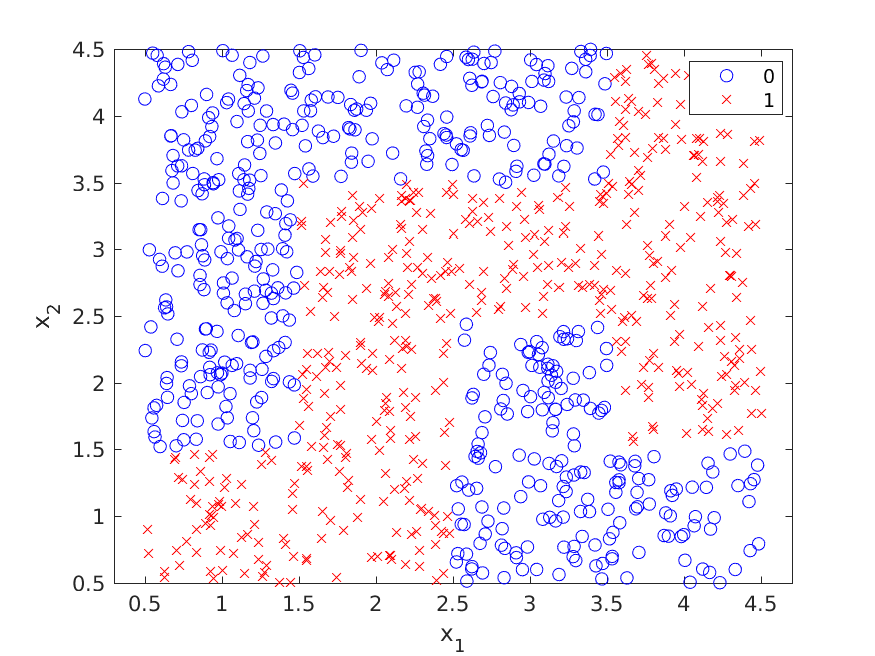
\includegraphics[width=0.8\textwidth]{1_4}
	\caption{Проверка в случайных точках входного пространства}
	\label{fig:1_4}
\end{center}
\end{figure}

\subsection{Решение с помощью 1-слойного персептрона}

%5. Попытайтесь решить задачу распознавания путем обучения 1-слойного персептрона на множестве входных примеров. Проанализируйте полученный результат.

Попробуем решить задачу распознование путем обучения 1-слойного персептрона. На рис. \ref{fig:1_5_1} изображено разбиение на 2 класса. Средняя ошибка при этом оказалась равна $0.4805$.

\begin{figure}[H]
\begin{center}
	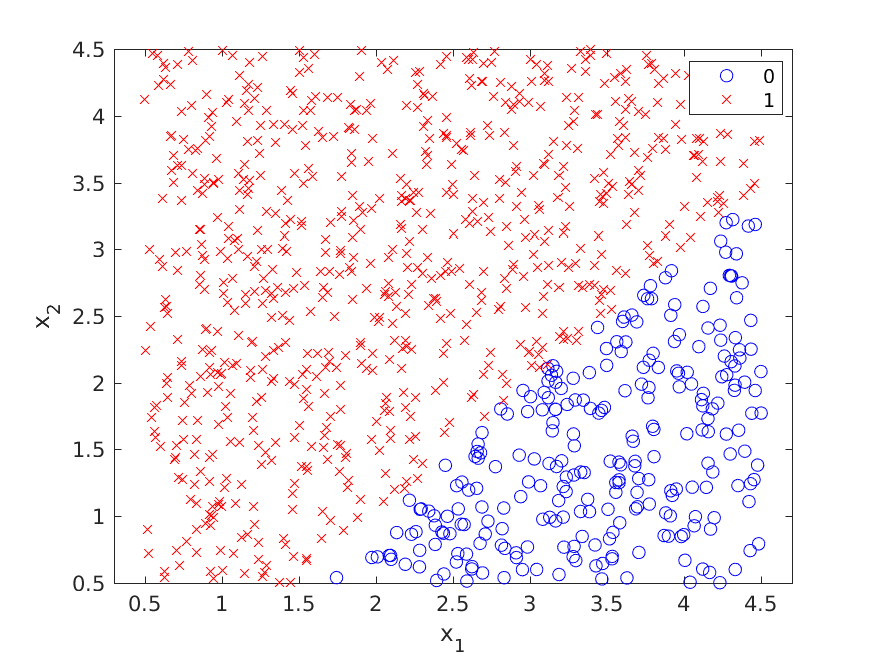
\includegraphics[width=0.8\textwidth]{1_5_1}
	\caption{Разбиение с помощью 1-слойного персептрона}
	\label{fig:1_5_1}
\end{center}
\end{figure}

На рис. \ref{fig:1_5_2} изображено значние ошибки в процессе обучения. Видно что оно колеблется, следовательно процесс обучения не сходится.

\begin{figure}[H]
\begin{center}
	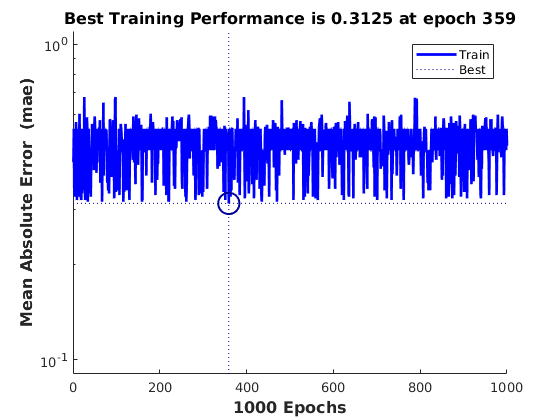
\includegraphics[width=0.8\textwidth]{1_5_2}
	\caption{Значние ошибки в процессе обучения}
	\label{fig:1_5_2}
\end{center}
\end{figure}

\section{Линейная функция}

\subsection{СДНФ}

Задана логическая функция:

\begin{equation*}
\begin{cases}
	y = f(X)\\
	X = [x_1, x_2, x_3, x_4, x_5]\\
	x_i \in \{0, 1\}\\
	y_i \in \{0, 1\}\\
	y(X) = 0, X \in \{ 5, 10, 13, 15, 16, 21, 24, 26 \}
\end{cases}
\end{equation*}

\begin{align*}
&\overline{x_1}\ \overline{x_2}\ x_3\ \overline{x_4}\ x_5 +
\overline{x_1}\ x_2\ \overline{x_3}\ x_4\ \overline{x_5} +
\overline{x_1}\ x_2\ x_3\ \overline{x_4}\ x_5 +
\overline{x_1}\ x_2\ x_3\ x_4\ x_5\ + \\
&x_1\ \overline{x_2}\ \overline{x_3}\ \overline{x_4}\ \overline{x_5} +
x_1\ \overline{x_2}\ x_3\ \overline{x_4}\ x_5 +
x_1\ x_2\ \overline{x_3}\ \overline{x_4}\ \overline{x_5} +
x_1\ x_2\ \overline{x_3}\ x_4\ \overline{x_5}
\end{align*}

%1.  Запишите выражение для вашей ЛФ в форме СДНФ.

\subsection{СДНФ в форме 2-слойного персептрона}

%2. Реализуйте полученную СДНФ в форме 2-слойного персептрона (net) в Matlab.

Логическая функция была реализована в форме 2-слойного персептрона. 

\subsection{Схема сети}

%3. Сгенерируйте схему командой gensim (net), проанализируйте ее и приведите в отчет.


На рис. \ref{fig:2_3} изображена схема, полученная при помощи команды \verb+gensim+.

\begin{figure}[H]
\begin{center}
	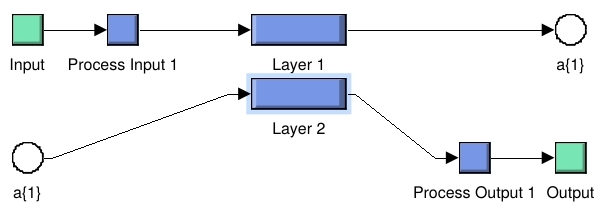
\includegraphics[width=0.8\textwidth]{2_3}
	\caption{Схема сети}
	\label{fig:2_3}
\end{center}
\end{figure}

\subsection{Проверка работы}

%4. Проверьте правильность работы полученной НС по таблице истинности.

На рис. \ref{fig:2_4} изображены выходные значения для 32 входных примеров. Выходные значения нейронной сети полностью совпали с таблицей истинности.

\begin{figure}[H]
\begin{center}
	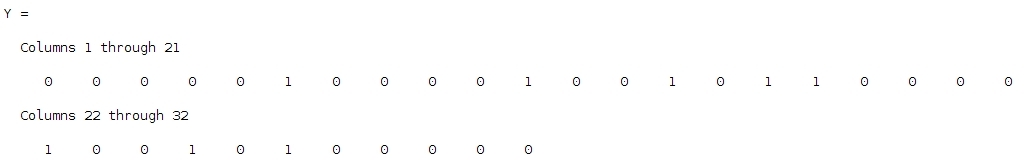
\includegraphics[width=1\textwidth]{2_4}
	\caption{Выходные значения}
	\label{fig:2_4}
\end{center}
\end{figure}

\subsection{Решение с помощью 1-слойного персептрона}

%5. Попробуйте обучить однослойный персептрон на Вашей функции, используя в качестве обучающей выборки фрагменты таблицы истинности. Проанализируйте результаты и посчитайте среднюю ошибку.	

Попробуем решить задачу путем обучения 1-слойного персептрона. На рис. \ref{fig:2_5} изображено значние ошибки в процессе обучения. Видно что оно колеблется, следовательно процесс обучения не сходится. Средняя ошибка при этом оказалась равна $0.3750$.

\begin{figure}[H]
\begin{center}
	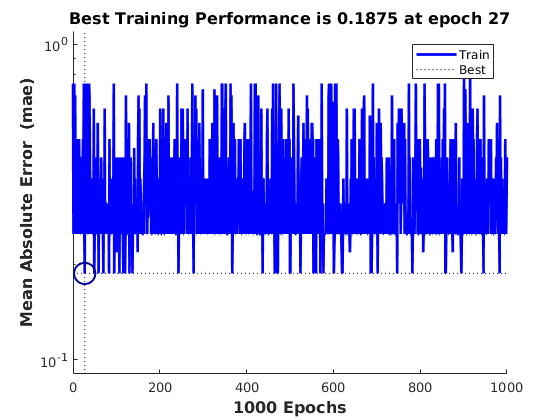
\includegraphics[width=0.8\textwidth]{2_5}
	\caption{Значние ошибки в процессе обучения}
	\label{fig:2_5}
\end{center}
\end{figure}

\section{Классификация 2 класссов}

\subsection{Набор входных и желаемых образов}

Сформируем набор входных и желаемых выходных образов для двух линейно-неразделимых классов. На рис. \ref{fig:3_1} входной набор изоражен на графике, при этом класс \verb+1+ выделен синей областью.

\begin{figure}[H]
\begin{center}
	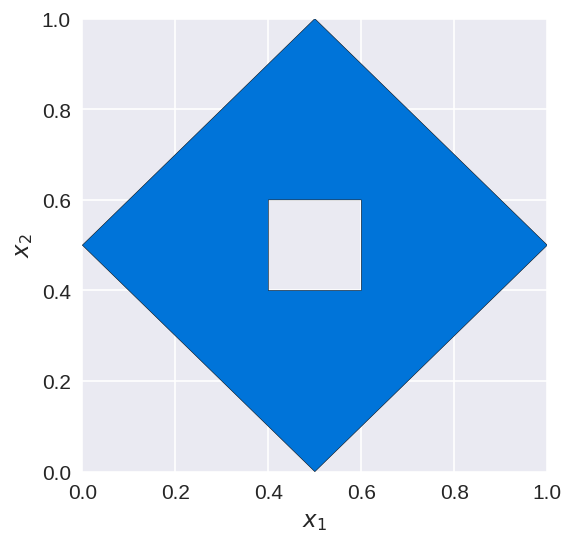
\includegraphics[scale=1]{3_1}
	\caption{Набор выходных и желаемых выходных образов}
	\label{fig:3_1}
\end{center}
\end{figure}

\subsection{Аналитическое решение}

%1. Запишите аналитическое выражение для функции, реализующей Ваше разбиение плоскости на 2 класса. Постройте график функции и разбиение плоскости на классы.
%2. Реализуйте полученную функцию в форме 2-х или 3-х слойного персептрона net в Matlab. 

\paragraph{Первый слой}
\begin{enumerate}
	\item $x_1 - x_2 + 1.5 = 0 \rightarrow y_{11}$
	\item $-x_1 + x_2 + 0.5 = 0 \rightarrow y_{12}$
	\item $-x_1 + x_2 - 0.5 = 0 \rightarrow y_{13}$
	\item $x_1 + x_2 - 0.5 = 0 \rightarrow y_{14}$
	\item $-x_1 + 0.4 = 0 \rightarrow y_{15}$
	\item $x_2 - 0.6 = 0 \rightarrow y_{16}$
	\item $x_1 - 0.6 = 0 \rightarrow y_{17}$
	\item $-x_2 + 0.4 = 0 \rightarrow y_{18}$
\end{enumerate}

\paragraph{Второй слой}
\begin{enumerate}
	\item $y_{11} + y_{12} + y_{13} + y_{14} - 3.5 = 0 \rightarrow y_{21}$
	\item $y_{15} + y_{16} + y_{17} + y_{18} - 3.5 = 0 \rightarrow y_{22}$
\end{enumerate}

\paragraph{Третий слой}
\begin{enumerate}
	\item $y = y_{21} - 2 y_{22} - 0.5$
\end{enumerate}

\subsection{Схема сети}

%3. Сгенерируйте схему командой gensim (net), проанализируйте ее и приведите в отчет.

На рис. \ref{fig:3_3} изображена схема, полученная при помощи команды \verb+gensim+.

\begin{figure}[H]
\begin{center}
	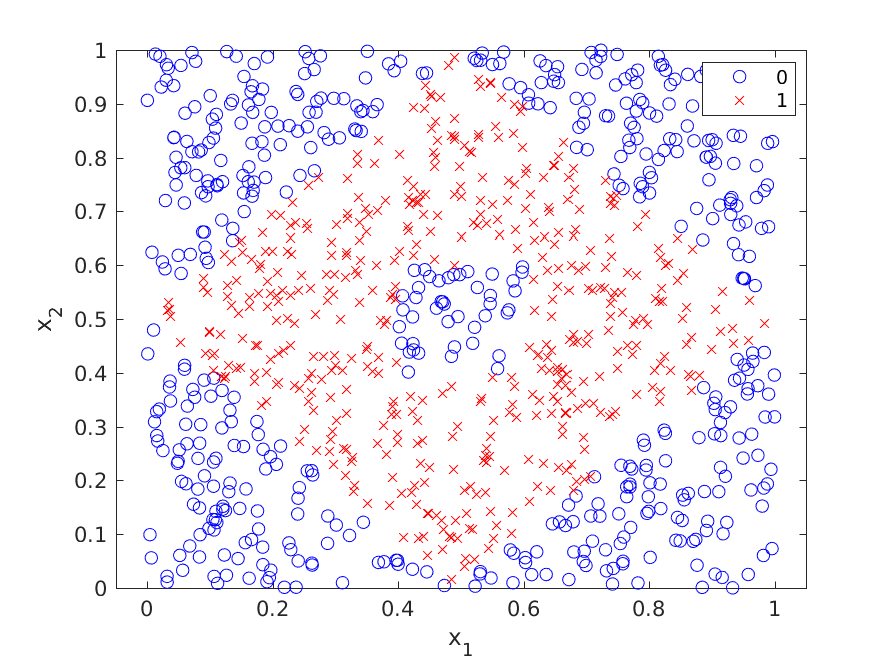
\includegraphics[width=0.8\textwidth]{3_3}
	\caption{Схема сети}
	\label{fig:3_3}
\end{center}
\end{figure}

\subsection{Проверка аналитического решения}

%4. Проверьте правильность работы полученной НС путем построения разбиения плоскости на классы, которое реализует персептрон.

На рис. \ref{fig:3_4} изображено разбиение случайных точек входного пространства на классы.

\begin{figure}[H]
\begin{center}
	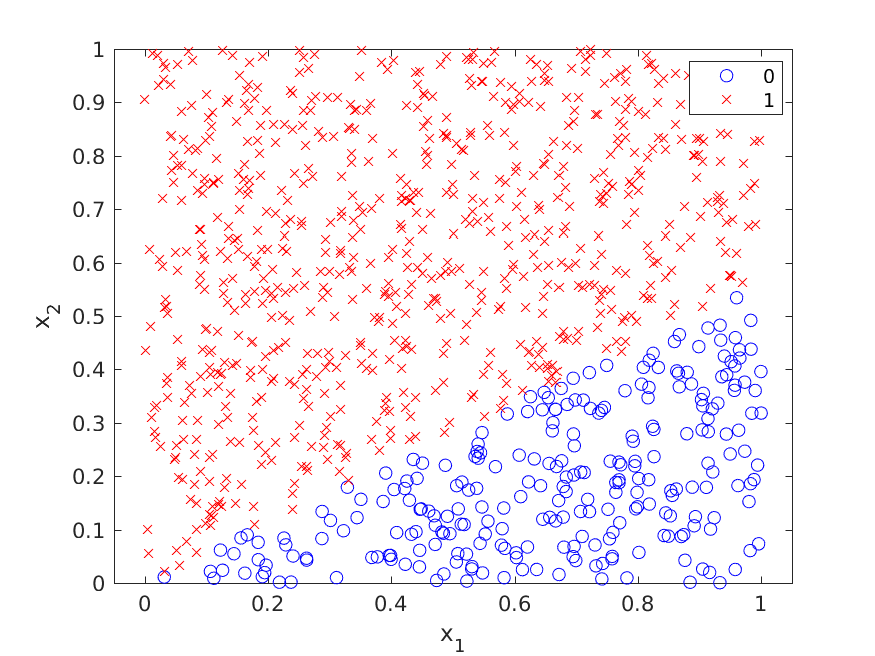
\includegraphics[width=0.8\textwidth]{3_4}
	\caption{Проверка в случайных точках входного пространства}
	\label{fig:3_4}
\end{center}
\end{figure}

\subsection{Решение с помощью 1-слойного персептрона}

%5. Попытайтесь решить задачу распознавания путем обучения 1-слойного персептрона на множестве входных примеров. Для этого вначале сформируйте обучающую выборку необходимого объема. 

Попробуем решить задачу распознование путем обучения 1-слойного персептрона. На рис. \ref{fig:3_5_1} изображено разбиение на 2 класса. Средняя ошибка при этом оказалась равна $0.5140$.

\begin{figure}[H]
\begin{center}
	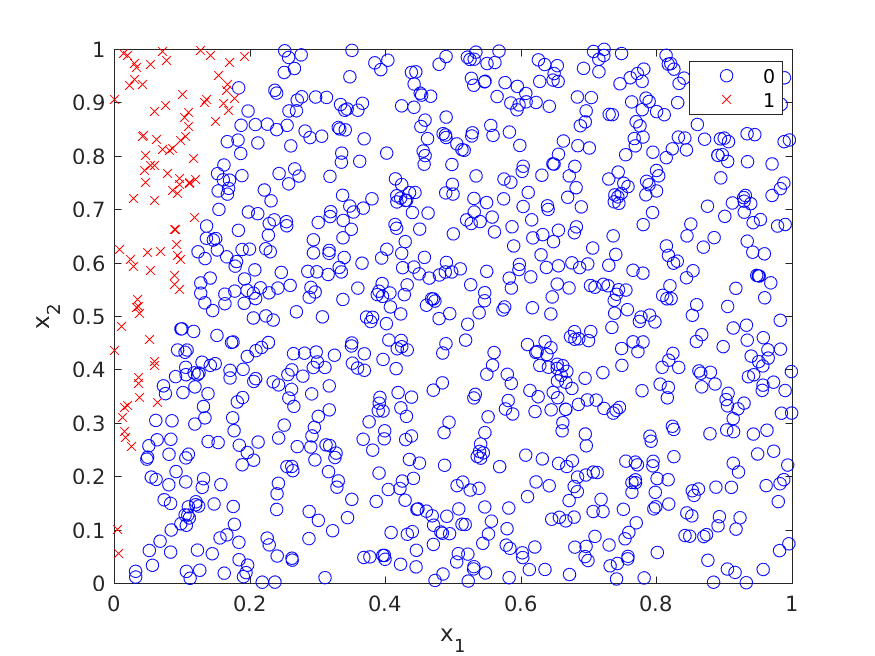
\includegraphics[width=0.8\textwidth]{3_5_1}
	\caption{Разбиение с помощью 1-слойного персептрона}
	\label{fig:3_5_1}
\end{center}
\end{figure}

На рис. \ref{fig:3_5_2} изображено значние ошибки в процессе обучения. Видно что оно колеблется, следовательно процесс обучения не сходится.

\begin{figure}[H]
\begin{center}
	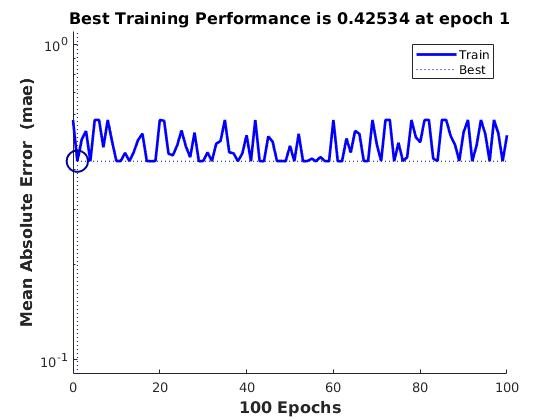
\includegraphics[width=0.8\textwidth]{3_5_2}
	\caption{Значние ошибки в процессе обучения}
	\label{fig:3_5_2}
\end{center}
\end{figure}

%\subsection{Анализ результатов}

%6. После обучения посчитайте среднюю ошибку, проанализируйте результаты – какую функцию реализует обученная сеть. 

\section{Классификация $N$ классов}

\subsection{Набор входных и желаемых образов}

Сформируем набор входных и желаемых выходных образов для двух линейно-неразделимых классов. На рис. \ref{fig:4_1} входной набор изоражен на графике, при этом каждый класс выделен свои цветом.

\begin{figure}[H]
\begin{center}
	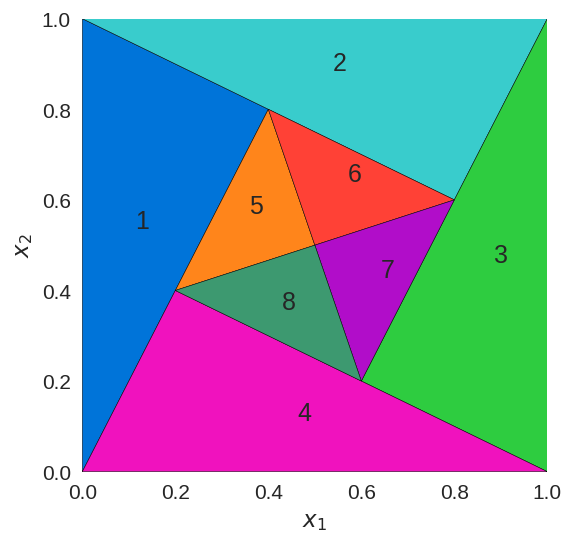
\includegraphics[scale=0.8]{4_1}
	\caption{Набор входных и желаемых выходных образов}
	\label{fig:4_1}
\end{center}
\end{figure}

\subsection{Аналитическое решение}

%1. Запишите аналитическое выражение для функции, реализующей Ваше разбиение плоскости на m классов. Постройте график с разбиением плоскости на m классов.
%2. Реализуйте полученную функцию в форме 2-х или 3-х слойного персептрона net в Matlab. 

Пронумеруем прямые и обединим и в фигуры. На рис. \ref{fig:4_2} прямые пронумерованы обозначены былым цветом.
\begin{figure}[H]
\begin{center}
	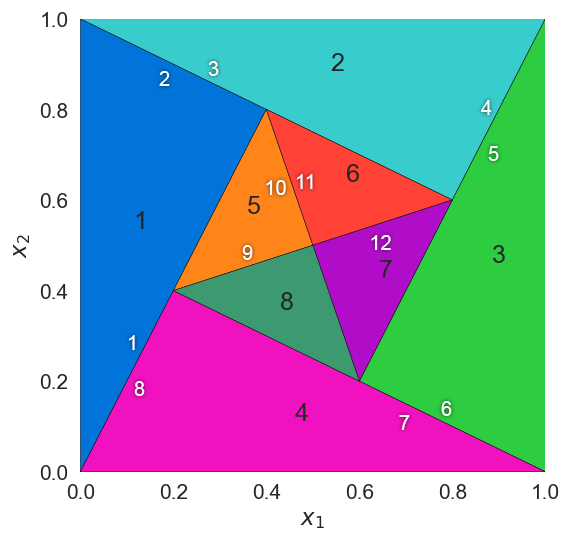
\includegraphics[scale=0.8]{4_2}
	\caption{Прямые, разбивающие плоскость на классы}
	\label{fig:4_2}
\end{center}
\end{figure}

Тогда классы ограничены следующими прямыми:

\begin{multicols}{4}
\begin{enumerate}[label=\arabic*)]
	\item 1, 2
	\item 3, 4
	\item 5, 6
	\item 7, 8
	\item 8, 9, 10
	\item 2, 9, 11
	\item 4, 11, 12
	\item 6, 10, 12
\end{enumerate}
\end{multicols}

Запишем уравнения прямых первого слоя сети:
\begin{multicols}{2}
\begin{enumerate}
	\item $-2 x_1 + x_2 = 0 \rightarrow y_{1,1}$
	\item $-0.5 x_1 - x_2 + 1 = 0 \rightarrow y_{1,2}$
	\item $0.5 x_1 + x_2 - 1 = 0 \rightarrow y_{1,3}$
	\item $-2 x_1 + x_2 + 1 = 0 \rightarrow y_{1,4}$
	\item $2 x_1 - x_2 - 1 = 0 \rightarrow y_{1,5}$
	\item $0.5 x_1 + x_2 - 0.5 = 0 \rightarrow y_{1,6}$
	\item $-0.5 x_1 - x_2 + 0.5 = 0 \rightarrow y_{1,7}$
	\item $2 x_1 - x_2 = 0 \rightarrow y_{1,8}$
	\item $-\frac{1}{3} x_1 + x_2 - \frac{1}{3} = 0 \rightarrow y_{1,9}$
	\item $-3 x_1 - x_2 + 2 = 0 \rightarrow y_{1,10}$
	\item $3 x_1 + x_2 - 2 = 0 \rightarrow y_{1,11}$
	\item $\frac{1}{3} x_1 - x_2 + \frac{1}{3} = 0 \rightarrow y_{1,12}$
\end{enumerate}
\end{multicols}

Запишем уравнения выходного слоя сети:
\begin{multicols}{2}
\begin{enumerate}
	\item $y_{1,1} + y_{1,2} - 1.5 = 0 \rightarrow y_{2,1}$
	\item $y_{1,3} + y_{1,4} - 1.5 = 0 \rightarrow y_{2,2}$
	\item $y_{1,5} + y_{1,6} - 1.5 = 0 \rightarrow y_{2,3}$
	\item $y_{1,7} + y_{1,8} - 1.5 = 0 \rightarrow y_{2,4}$
	\item $y_{1,8} + y_{1,9} + y_{1,10} - 2.5 = 0 \rightarrow y_{2,5}$
	\item $y_{1,3} + y_{1,9} + y_{1,11} - 2.5 = 0 \rightarrow y_{2,6}$
	\item $y_{1,4} + y_{1,11} + y_{1,12} - 2.5 = 0 \rightarrow y_{2,7}$
	\item $y_{1,6} + y_{1,10} + y_{1,12} - 2.5 = 0 \rightarrow y_{2,8}$
\end{enumerate}
\end{multicols}

\subsection{Схема сети}

%3. Сгенерируйте схему командой gensim (net), проанализируйте ее и приведите в отчет.

На рис. \ref{fig:4_3} изображена схема, полученная при помощи команды \verb+gensim+.

\begin{figure}[H]
\begin{center}
	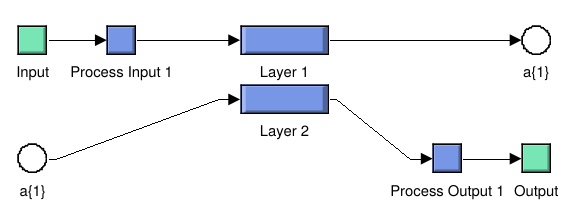
\includegraphics[width=0.8\textwidth]{4_3}
	\caption{Схема сети}
	\label{fig:4_3}
\end{center}
\end{figure}

\subsection{Проверка аналитического решения}

%4. Проверьте правильность работы полученной НС путем построения разбиения плоскости на классы, которое реализует персептрон.

На рис. \ref{fig:4_4} изображено разбиение случайных точек входного пространства на классы.

\begin{figure}[H]
\begin{center}
	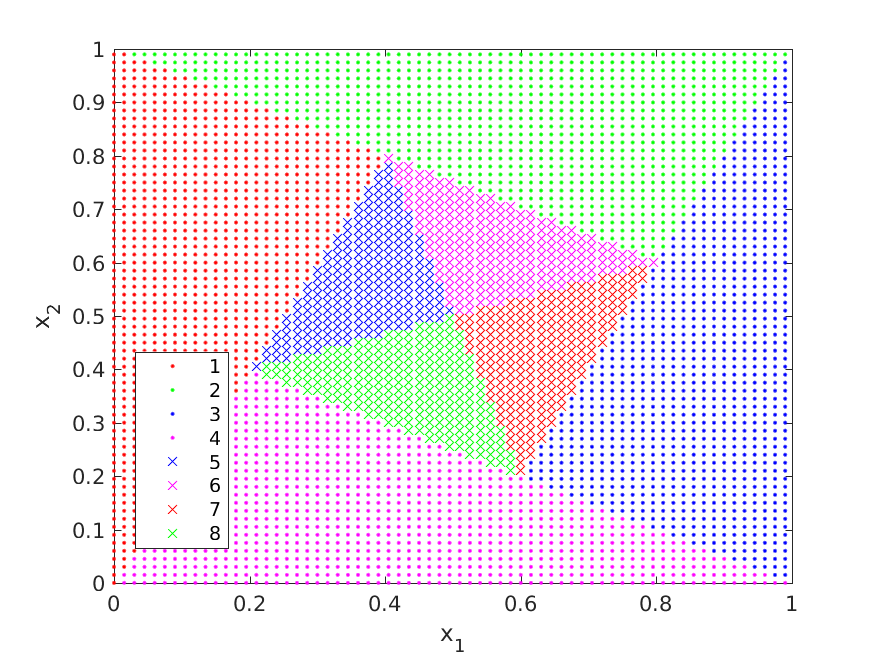
\includegraphics[width=0.9\textwidth]{4_4}
	\caption{Проверка в случайных точках входного пространства}
	\label{fig:4_4}
\end{center}
\end{figure}

\section{Классификация данных на плоскости}

\subsection{Генерация выборок}

%1. Сгенерировать две выборки X1-Y1, X2-Y2, представляющих собой множество двух линейно разделимых и линейно-неразделимых классов на плоскости.

На рис. \ref{fig:5_1_1} изображена выборка линейно-разделимых классов на плоскости.

\begin{figure}[H]
\begin{center}
	
\includegraphics[width=0.85\textwidth]{5_1_1}
	\caption{Выборка линейно-разделимых классов на плоскости}
	\label{fig:5_1_1}
\end{center}
\end{figure}

На рис. \ref{fig:5_1_2} изображена выборка линейно-неразделимых классов на плоскости.

\begin{figure}[H]
\begin{center}
	
\includegraphics[width=0.85\textwidth]{5_1_2}
	\caption{Выборка линейно-неразделимых классов на плоскости}
	\label{fig:5_1_2}
\end{center}
\end{figure}

\subsection{Решение с помощью 1-слойного перспетрона}

В таблице \ref{tab:6_2_1} приведена сравнительная таблица, содержащая среднее количество эпох, требуемых перспетрону для достижения нулевой ошибки на первом наборе данных в зависимости от функций обучения. Из таблицы видно, что в среднем обучение происходило быстрее всего при обучении с нормализацией \verb+learnpn+ с применением последовательного случайного алгоритма обучения \verb+trainr+.

\begin{table}[H]
\begin{center}
	\def\tabcolsep{15pt}
	\caption{Среднее количество эпох}
	\label{tab:6_2_1}
	\begin{tabular}{|c|c|c|c|}
		\hline
		 & \verb+trainc+ & \verb+trainr+ & \verb+trainb+ \\
		\hline
		\verb+learnp+ & 15.4 & 4.6 & 11.0 \\
		\hline
		\verb+learnpn+ & 14.4 & 3.8 & 11.0 \\
		\hline
	\end{tabular}
\end{center}
\end{table} 

На рисунках \ref{fig:5_2_1} -- \ref{fig:5_2_3} изображены характеристики обучения в зависимости от номера эпохи для некоторого обучения с использованием \verb+learnpn+ и \verb+trainr+.
\begin{figure}[H]
\begin{center}
	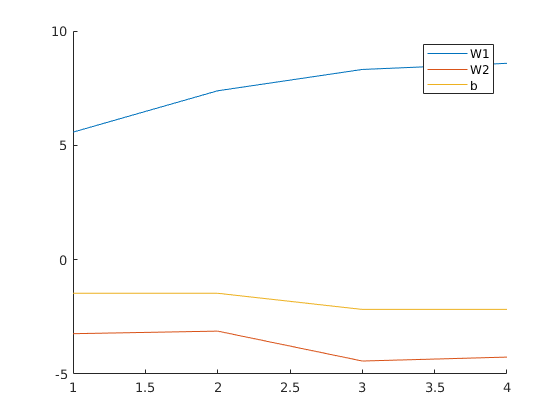
\includegraphics[width=0.85\textwidth]{5_2_1}
	\caption{Динамика изменения весовых коэффициентов}
	\label{fig:5_2_1}
\end{center}
\end{figure}
\begin{figure}[H]
\begin{center}
	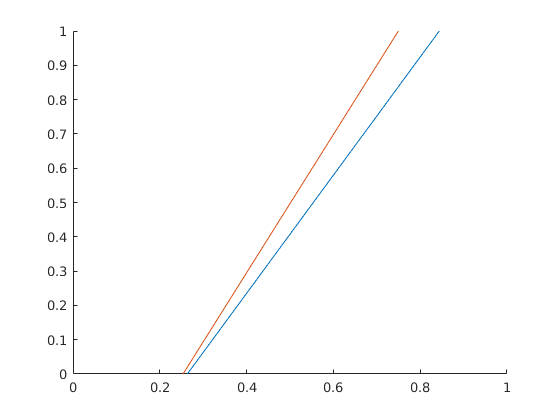
\includegraphics[width=0.85\textwidth]{5_2_2}
	\caption{Динамика (эволюция) прямых, реализуемых персептроном}
	\label{fig:5_2_2}
\end{center}
\end{figure}
\begin{figure}[H]
\begin{center}
	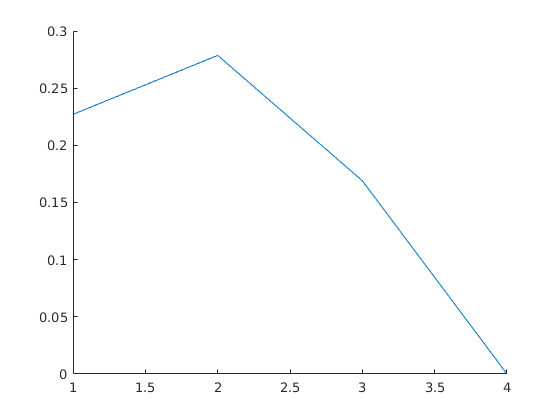
\includegraphics[width=0.85\textwidth]{5_2_3}
	\caption{Динамика значения ошибки}
	\label{fig:5_2_3}
\end{center}
\end{figure}

В таблице \ref{tab:6_2_2} приведена сравнительная таблица, содержащая среднее количество эпох, требуемых перспетрону для достижения ошибки $0.13$ на втором наборе данных в зависимости от функций обучения. Из таблицы видно, что в среднем обучение происходило быстрее всего при обучении с нормализацией \verb+learnpn+ с применением последовательного случайного алгоритма обучения \verb+trainr+. Средняя ошибка при этом оказалась равна $0.1292$.

\begin{table}[H]
\begin{center}
	\def\tabcolsep{15pt}
	\caption{Среднее количество эпох}
	\label{tab:6_2_2}
	\begin{tabular}{|c|c|c|c|}
		\hline
		 & \verb+trainc+ & \verb+trainr+ & \verb+trainb+ \\
		\hline
		\verb+learnp+ & 8.4 & 1.4 & 12.0 \\
		\hline
		\verb+learnpn+ & 12.2 & 1.0 & 12.0 \\
		\hline
	\end{tabular}
\end{center}
\end{table} 

На рис. \ref{fig:5_2_4} и \ref{fig:5_2_5} приведены примеры классификации с помощью 1-слойного персептрона после обучения.
\begin{figure}[H]
\begin{center}
	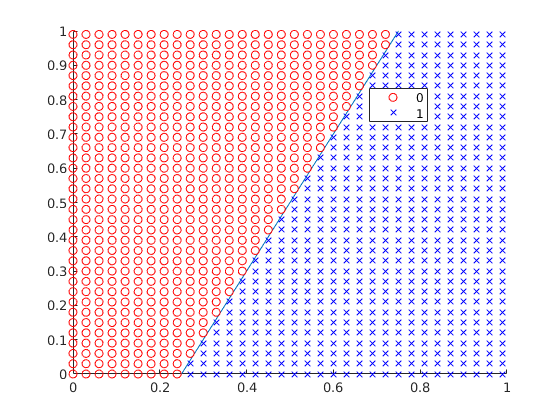
\includegraphics[width=0.85\textwidth]{5_2_4}
	\caption{Классификация линейно-разделимых классов на плоскости}
	\label{fig:5_2_4}
\end{center}
\end{figure}
\vspace{-1cm}
\begin{figure}[H]
\begin{center}
	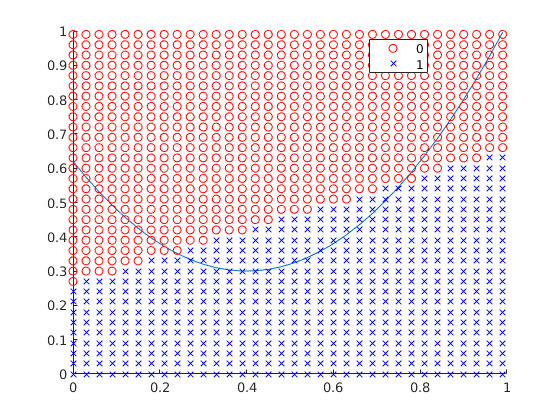
\includegraphics[width=0.85\textwidth]{5_2_5}
	\caption{Классификация линейно-неразделимых классов на плоскости}
	\label{fig:5_2_5}
\end{center}
\end{figure}

\section{Выводы}

В данной работе были приобретены навыки построения и обучения персептронов для различных областей применения. Была изучена архитектура персептрона и специальные функции для создания персептрона. Была произведена как ручная настройка весов при помощи аналитического решения, так и использованы функции для обучения персептрона. 

\end{document}